
\begin{figure}[t]
\centering
% \begin{tikzpicture}[->, >=stealth,font=\small]
%   \tikzstyle{cell} = [rectangle,draw=black,minimum width=40,minimum
%   height = 15,node distance=15]
%   \tikzstyle{register} = [rectangle,draw=black,rounded corners];
%   \node[register,name=idxhead] {index\_head};
%   \node[register,name=idxfree, below of=idxhead] {index\_free = 2};


%   \node[cell,name=idx0, right of=idxhead,xshift=40] {$I_0$};
%   \node[cell,name=idx1, below of=idx0] {$I_1$ (free)};
%   \node[cell,name=idx2, below of=idx1] {$I_2$ (free)};
%   \node[cell,name=idx3, below of=idx2] {$I_3$};
%   \node[cell,name=idx4, below of=idx3] {$I_4$};
%   \node[above of=idx0,yshift=-10] {\underline{Index Array}};

%   \node[cell,name=dat0, right of=idx0,xshift=40] {$D_{\rm free}$};
%   \node[cell,name=dat1, below of=dat0] {$D_{18}$};
%   \node[cell,name=dat2, below of=dat1] {$D_{19}$};
%   \node[cell,name=dat3, below of=dat2] {$D_{20}$};
%   \node[cell,name=dat4, below of=dat3] {$D_{\rm free}$};
%   \node[above of=dat0,yshift=-10] {\underline{Data Array}};

%   \node[register,name=dathead,right of=dat2,xshift=40] {data\_head};
%   \node[register,name=datfree,below of=dathead] {data\_free = $n$};
%   \node[register,name=datfree,above of=dathead] {Seq. Num. = 20};


%   \path (idxhead) edge (idx1.west);
%   \path (idx3.east) edge (dat1.west);
%   \path (idx4.east) edge (dat2.west);
%   \path (idx0.east) edge (dat3.west);
%   \path (dathead) edge (dat4.east);
% \end{tikzpicture}

\ovalbox{
  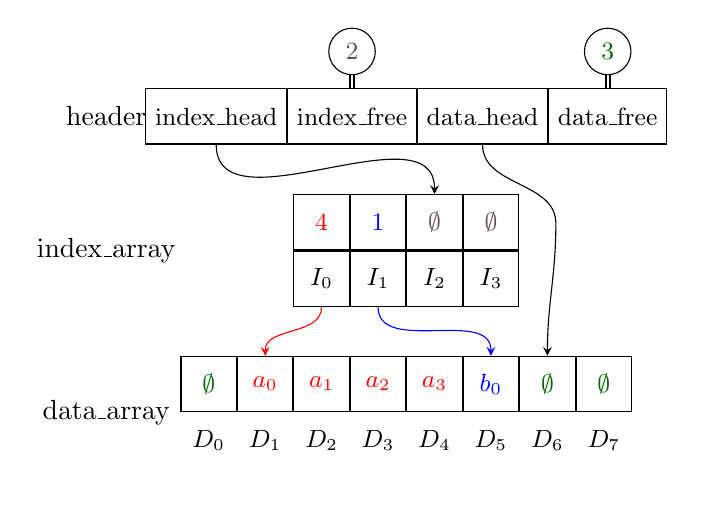
\begin{tikzpicture}
  \tikzstyle{cell} = [rectangle,minimum height=2.0em,minimum
  width=2.00em, font=\small,draw=black]
  \tikzstyle{vcell} = [rectangle,minimum height=2.0em,minimum
  width=2.00em, font=\small,draw=white]

  \tikzstyle{ref} =[->, >=stealth,out=-90,in=90]

  \node [matrix,nodes=draw] (header)
  {
    \node[cell,name=idxhead]{index\_head}; &
    \node[cell,name=idxfree]{index\_free}; &
    \node[cell,name=dathead]{data\_head}; &
    \node[cell,name=datfree]{data\_free};\\
  };
  \node[draw,font=\small,circle,above
  of=idxfree,name=vif,color=pink!40!black,draw=black,yshift=-0.5em] {2};
  \node[draw,font=\small,circle,above
  of=datfree,name=vdf,color=green!40!black,draw=black,yshift=-.5em] {3};

  \node [matrix,below of=header,yshift=-2.0em] (index)
  {
    \node[cell,name=n0,color=red,draw=black]{$4$}; &
    \node[cell,name=n1,color=blue,draw=black]{$1$}; &
    \node[cell,name=n2,color=pink!40!black,draw=black]{$\emptyset$}; &
    \node[cell,name=n3,color=pink!40!black,draw=black]{$\emptyset$}; \\
    \node[cell,name=i0,font=\small]{$I_0$}; &
    \node[cell,name=i1,font=\small]{$I_1$}; &
    \node[cell,name=i2,font=\small]{$I_2$}; &
    \node[cell,name=i3,font=\small]{$I_3$}; \\
  };
  \node [matrix,below of=index,yshift=-3.0em] (data)
  {
    \node[cell,name=v0,color=green!40!black,draw=black]{$\emptyset$}; &
    \node[cell,name=v1,color=red, draw=black]{$a_0$}; &
    \node[cell,name=v2,color=red,draw=black]{$a_1$}; &
    \node[cell,name=v3,color=red,draw=black]{$a_2$}; &
    \node[cell,name=v4,color=red,draw=black]{$a_3$}; &
    \node[cell,name=v5,color=blue,draw=black]{$b_0$}; &
    \node[cell,name=v6,color=green!40!black,draw=black]{$\emptyset$}; &
    \node[cell,name=v7,color=green!40!black,draw=black]{$\emptyset$}; \\
    \node[vcell,name=d0]{$D_0$}; &
    \node[vcell,name=d1]{$D_1$}; &
    \node[vcell,name=d2]{$D_2$}; &
    \node[vcell,name=d3]{$D_3$}; &
    \node[vcell,name=d4]{$D_4$}; &
    \node[vcell,name=d5]{$D_5$}; &
    \node[vcell,name=d6]{$D_6$}; &
    \node[vcell,name=d7]{$D_7$}; \\
  };
  \node[name=hlabel,left of=header,xshift=-8em] {header};
  \node[name=ilabel,left of=index,xshift=-8em] {index\_array};
  \node[name=dlabel,left of=data,xshift=-8em] {data\_array};
  %\path (hlabel) edge[dotted] (idxhead);
  %\path (ilabel) edge[dotted] (i0);
  %\path (dlabel) edge[dotted] (d0);

  \path (idxhead.south) edge[ref,out=-90,in=90] (n2.north);
  \node[coordinate,name=d0dot,right of=i3,xshift=-0.5em,yshift=2em] {};
  \path (dathead) edge[out=-90,in=90] (d0dot);
  \path (d0dot) edge[ref,out=-90,in=90] (v6);

  \path (i1) edge[ref,color=blue] (v5);
  \path (i0) edge[ref,color=red] (v1);

  \path (idxfree) edge[double,thick] (vif);
  \path (datfree) edge[double,thick] (vdf);

\end{tikzpicture}
}
\caption{Logical Memory Structure for an Ach shared memory file. In
  this example, $I_0$ points to a four byte message starting at $D_1$,
  and $I_1$ points to a one byte message starting at $D_5$.  The next
  inserted message will use index cell $I_2$ and start at $D_6$.
  There are two free index cells and three free data bytes.  Both
  arrays are circular and wrap around when the end is reached.}
\label{fig:chanstruct}
\vspace{-15pt}
\end{figure}




